%===============================================================================
% LaTeX sjabloon voor de bachelorproef toegepaste informatica aan HOGENT
% Meer info op https://github.com/HoGentTIN/latex-hogent-report
%===============================================================================

\documentclass[dutch,dit,thesis]{hogentreport}

% TODO:
% - If necessary, replace the option `dit`' with your own department!
%   Valid entries are dbo, dbt, dgz, dit, dlo, dog, dsa, soa
% - If you write your thesis in English (remark: only possible after getting
%   explicit approval!), remove the option "dutch," or replace with "english".

\usepackage{lipsum} % For blind text, can be removed after adding actual content

%% Pictures to include in the text can be put in the graphics/ folder
\graphicspath{{../graphics/}}

%% For source code highlighting, requires pygments to be installed
%% Compile with the -shell-escape flag!
%% \usepackage[chapter]{minted}
%% If you compile with the make_thesis.{bat,sh} script, use the following
%% import instead:
\usepackage[chapter,outputdir=../output]{minted}
\usemintedstyle{solarized-light}

%% Formatting for minted environments.
\setminted{%
    autogobble,
    frame=lines,
    breaklines,
    linenos,
    tabsize=4
}

%% Ensure the list of listings is in the table of contents
\renewcommand\listoflistingscaption{%
    \IfLanguageName{dutch}{Lijst van codefragmenten}{List of listings}
}
\renewcommand\listingscaption{%
    \IfLanguageName{dutch}{Codefragment}{Listing}
}
\renewcommand*\listoflistings{%
    \cleardoublepage\phantomsection\addcontentsline{toc}{chapter}{\listoflistingscaption}%
    \listof{listing}{\listoflistingscaption}%
}

% Other packages not already included can be imported here

%%---------- Document metadata -------------------------------------------------
% TODO: Replace this with your own information
\author{Keoma Plovie}
\supervisor{Mevr. C. De Leenheer}
\cosupervisor{Dhr. A. Boel}
\title[]%
    {Pose Estimation als basis voor effectieve feedback in
    krachttraining: een mobiele oplossing.}
\academicyear{\advance\year by -1 \the\year--\advance\year by 1 \the\year}
\examperiod{1}
\degreesought{\IfLanguageName{dutch}{Professionele bachelor in de toegepaste informatica}{Bachelor of applied computer science}}
\partialthesis{false} %% To display 'in partial fulfilment'
%\institution{Internshipcompany BVBA.}

%% Add global exceptions to the hyphenation here
\hyphenation{back-slash}

%% The bibliography (style and settings are  found in hogentthesis.cls)
\addbibresource{bachproef.bib}            %% Bibliography file
\addbibresource{../voorstel/voorstel.bib} %% Bibliography research proposal
\defbibheading{bibempty}{}

%% Prevent empty pages for right-handed chapter starts in twoside mode
\renewcommand{\cleardoublepage}{\clearpage}

\renewcommand{\arraystretch}{1.2}

%% Content starts here.
\begin{document}

%---------- Front matter -------------------------------------------------------

\frontmatter

\hypersetup{pageanchor=false} %% Disable page numbering references
%% Render a Dutch outer title page if the main language is English
\IfLanguageName{english}{%
    %% If necessary, information can be changed here
    \degreesought{Professionele Bachelor toegepaste informatica}%
    \begin{otherlanguage}{dutch}%
       \maketitle%
    \end{otherlanguage}%
}{}

%% Generates title page content
\maketitle
\hypersetup{pageanchor=true}

%%=============================================================================
%% Voorwoord
%%=============================================================================

\chapter*{\IfLanguageName{dutch}{Woord vooraf}{Preface}}%
\label{ch:voorwoord}

%% TODO:
%% Het voorwoord is het enige deel van de bachelorproef waar je vanuit je
%% eigen standpunt (``ik-vorm'') mag schrijven. Je kan hier bv. motiveren
%% waarom jij het onderwerp wil bespreken.
%% Vergeet ook niet te bedanken wie je geholpen/gesteund/... heeft

Mijn interesse in de combinatie van sport en technologie is deels ingegeven door persoonlijke ervaringen. 
Vroeger liep ik zelf een blessure op door het verkeerd uitvoeren van oefeningen, wat mij bewust maakte van het belang van correcte begeleiding tijdens het sporten. 
Dit inspireerde mij om in mijn bachelorproef te onderzoeken hoe digitale technologieën kunnen bijdragen aan het verbeteren van de uitvoering van oefeningen en zo blessures te voorkomen.

Ik wil mijn copromotor, Arno Boel, en mijn stageplaats Delaware van harte bedanken. 
Dankzij hun begeleiding en de mogelijkheid om me te verdiepen in progressieve webapplicaties en AI-modellen in de browser, kon ik mijn technische kennis verrijken en toepassen binnen dit project.

Daarnaast ben ik mijn promotor, Chloé De Leenheer, zeer dankbaar voor haar waardevolle feedback en positiviteit, die mij geholpen hebben om deze bachelorproef tot een goed einde te brengen.

\lipsum[1-2]
%%=============================================================================
%% Samenvatting
%%=============================================================================

% TODO: De "abstract" of samenvatting is een kernachtige (~ 1 blz. voor een
% thesis) synthese van het document.
%
% Een goede abstract biedt een kernachtig antwoord op volgende vragen:
%
% 1. Waarover gaat de bachelorproef?
% 2. Waarom heb je er over geschreven?
% 3. Hoe heb je het onderzoek uitgevoerd?
% 4. Wat waren de resultaten? Wat blijkt uit je onderzoek?
% 5. Wat betekenen je resultaten? Wat is de relevantie voor het werkveld?
%
% Daarom bestaat een abstract uit volgende componenten:
%
% - inleiding + kaderen thema
% - probleemstelling
% - (centrale) onderzoeksvraag
% - onderzoeksdoelstelling
% - methodologie
% - resultaten (beperk tot de belangrijkste, relevant voor de onderzoeksvraag)
% - conclusies, aanbevelingen, beperkingen
%
% LET OP! Een samenvatting is GEEN voorwoord!

%%---------- Nederlandse samenvatting -----------------------------------------
%
% TODO: Als je je bachelorproef in het Engels schrijft, moet je eerst een
% Nederlandse samenvatting invoegen. Haal daarvoor onderstaande code uit
% commentaar.
% Wie zijn bachelorproef in het Nederlands schrijft, kan dit negeren, de inhoud
% wordt niet in het document ingevoegd.

\IfLanguageName{english}{%
\selectlanguage{dutch}
\chapter*{Samenvatting}
\selectlanguage{english}
}{}

%%---------- Samenvatting -----------------------------------------------------
% De samenvatting in de hoofdtaal van het document

\chapter*{\IfLanguageName{dutch}{Samenvatting}{Abstract}}

Deze bachelorproef richt zich op het ontwikkelen van een mobiele applicatie die personal trainers en fitnesscoaches ondersteunt bij het geven van nauwkeurige feedback op de uitvoering van krachttrainingsoefeningen. 
Door het toenemende aantal mensen dat sport en traint op afstand, ontstaat er een groeiende behoefte aan digitale hulpmiddelen die bewegingen kunnen analyseren en vergelijken met referentiemateriaal om zo blessures door foutieve uitvoering te voorkomen.

De centrale onderzoeksvraag luidt: hoe kan een applicatie ontwikkeld worden die de bewegingspatronen van cliënten effectief analyseert en vergelijkt met referentievideo’s om bruikbare feedback te geven? Om deze vraag te beantwoorden is het onderzoek opgedeeld in meerdere fasen. 
Eerst is een literatuurstudie uitgevoerd om de meest geschikte pose estimation-technologieën en relevante parameters voor bewegingsvergelijking te identificeren. 
Vervolgens werd een dataset samengesteld met videobeelden van correcte en incorrecte oefeningsuitvoeringen. 
Op basis van deze data is een analysekader ontwikkeld dat automatisch lichaamshoeken berekent en vergelijkt met behulp van algoritmen.

Het resultaat is een proof-of-concept mobiele applicatie die videobeelden van krachttrainingsoefeningen analyseert, vergelijkt met referentiemateriaal en realtime feedback geeft over de technische uitvoering. 
Evaluatie toonde aan dat het systeem in staat is om bewegingsverschillen te detecteren en bruikbare feedback te genereren, wat bijdraagt aan het verbeteren van trainingsresultaten en het voorkomen van blessures.



%---------- Inhoud, lijst figuren, ... -----------------------------------------

\tableofcontents

% In a list of figures, the complete caption will be included. To prevent this,
% ALWAYS add a short description in the caption!
%
%  \caption[short description]{elaborate description}
%
% If you do, only the short description will be used in the list of figures

\listoffigures

% If you included tables and/or source code listings, uncomment the appropriate
% lines.
\listoftables

\listoflistings

% Als je een lijst van afkortingen of termen wil toevoegen, dan hoort die
% hier thuis. Gebruik bijvoorbeeld de ``glossaries'' package.
% https://www.overleaf.com/learn/latex/Glossaries

%---------- Kern ---------------------------------------------------------------

\mainmatter{}

% De eerste hoofdstukken van een bachelorproef zijn meestal een inleiding op
% het onderwerp, literatuurstudie en verantwoording methodologie.
% Aarzel niet om een meer beschrijvende titel aan deze hoofdstukken te geven of
% om bijvoorbeeld de inleiding en/of stand van zaken over meerdere hoofdstukken
% te verspreiden!

%%=============================================================================
%% Inleiding
%%=============================================================================

\chapter{\IfLanguageName{dutch}{Inleiding}{Introduction}}%
\label{ch:inleiding}

De inleiding moet de lezer net genoeg informatie verschaffen om het onderwerp te begrijpen en in te zien waarom de onderzoeksvraag de moeite waard is om te onderzoeken. In de inleiding ga je literatuurverwijzingen beperken, zodat de tekst vlot leesbaar blijft. Je kan de inleiding verder onderverdelen in secties als dit de tekst verduidelijkt. Zaken die aan bod kunnen komen in de inleiding~\autocite{Pollefliet2011}:

\begin{itemize}
  \item context, achtergrond
  \item afbakenen van het onderwerp
  \item verantwoording van het onderwerp, methodologie
  \item probleemstelling
  \item onderzoeksdoelstelling
  \item onderzoeksvraag
  \item \ldots
\end{itemize}

\section{\IfLanguageName{dutch}{Probleemstelling}{Problem Statement}}%
\label{sec:probleemstelling}

Uit je probleemstelling moet duidelijk zijn dat je onderzoek een meerwaarde heeft voor een concrete doelgroep. De doelgroep moet goed gedefinieerd en afgelijnd zijn. Doelgroepen als ``bedrijven,'' ``KMO's'', systeembeheerders, enz.~zijn nog te vaag. Als je een lijstje kan maken van de personen/organisaties die een meerwaarde zullen vinden in deze bachelorproef (dit is eigenlijk je steekproefkader), dan is dat een indicatie dat de doelgroep goed gedefinieerd is. Dit kan een enkel bedrijf zijn of zelfs één persoon (je co-promotor/opdrachtgever).

\section{\IfLanguageName{dutch}{Onderzoeksvraag}{Research question}}%
\label{sec:onderzoeksvraag}

Wees zo concreet mogelijk bij het formuleren van je onderzoeksvraag. Een onderzoeksvraag is trouwens iets waar nog niemand op dit moment een antwoord heeft (voor zover je kan nagaan). Het opzoeken van bestaande informatie (bv. ``welke tools bestaan er voor deze toepassing?'') is dus geen onderzoeksvraag. Je kan de onderzoeksvraag verder specifiëren in deelvragen. Bv.~als je onderzoek gaat over performantiemetingen, dan 

\section{\IfLanguageName{dutch}{Onderzoeksdoelstelling}{Research objective}}%
\label{sec:onderzoeksdoelstelling}

Wat is het beoogde resultaat van je bachelorproef? Wat zijn de criteria voor succes? Beschrijf die zo concreet mogelijk. Gaat het bv.\ om een proof-of-concept, een prototype, een verslag met aanbevelingen, een vergelijkende studie, enz.

\section{\IfLanguageName{dutch}{Opzet van deze bachelorproef}{Structure of this bachelor thesis}}%
\label{sec:opzet-bachelorproef}

% Het is gebruikelijk aan het einde van de inleiding een overzicht te
% geven van de opbouw van de rest van de tekst. Deze sectie bevat al een aanzet
% die je kan aanvullen/aanpassen in functie van je eigen tekst.

De rest van deze bachelorproef is als volgt opgebouwd:

In Hoofdstuk~\ref{ch:stand-van-zaken} wordt een overzicht gegeven van de stand van zaken binnen het onderzoeksdomein, op basis van een literatuurstudie.

In Hoofdstuk~\ref{ch:methodologie} wordt de methodologie toegelicht en worden de gebruikte onderzoekstechnieken besproken om een antwoord te kunnen formuleren op de onderzoeksvragen.

% TODO: Vul hier aan voor je eigen hoofstukken, één of twee zinnen per hoofdstuk

In Hoofdstuk~\ref{ch:conclusie}, tenslotte, wordt de conclusie gegeven en een antwoord geformuleerd op de onderzoeksvragen. Daarbij wordt ook een aanzet gegeven voor toekomstig onderzoek binnen dit domein.
\chapter{\IfLanguageName{dutch}{Stand van zaken}{State of the art}}%
\label{ch:stand-van-zaken}

% Tip: Begin elk hoofdstuk met een paragraaf inleiding die beschrijft hoe
% dit hoofdstuk past binnen het geheel van de bachelorproef. Geef in het
% bijzonder aan wat de link is met het vorige en volgende hoofdstuk.

% Pas na deze inleidende paragraaf komt de eerste sectiehoofding.

\section{\IfLanguageName{dutch}{Krachttraining}{Powerlifting}}%
\label{sec:krachttraining}

Krachttraining omvat intensieve oefeningen die het lichaam blootstellen aan hoge fysieke eisen en zware belastingen. 
Dit kan leiden tot blessures ten gevolge van overbelasting, verkeerde liftingtechnieken en onvoldoende rust.
De meeste blessures treden op tijdens de uitvoering van de squat, bench press en deadlift.  
Volgens \textcite{BengtssonEtAl2018} is het essentieel om de liftingtechniek te analyseren en te optimaliseren, evenals de trainingsbelasting en rusttijden, om het risico op blessures te verminderen.

\section{\IfLanguageName{dutch}{Artificiële Intelligentie}{Artificial Intelligence}}%
\label{sec:artificiële-intelligentie}

Artificiële Intelligentie (AI) is een dynamisch en snel evoluerend vakgebied dat zich richt op het ontwikkelen van systemen die taken kunnen uitvoeren die normaal gesproken menselijke intelligentie vereisen, zoals leren, probleemoplossing en besluitvorming \autocite{SharifaniEtAl2023}.

Het doel is om machines te ontwikkelen die autonoom kunnen functioneren in complexe en dynamische omgevingen \autocite{Kouassi2023}.

AI als vakgebied is al meer dan 65 jaar in ontwikkeling en heeft zich inmiddels diep genesteld in ons dagelijks leven. Het speelt immers een curicale rol in sectoren zoals gezondheidszorg, transport, onderwijs en industrie, en wordt gezien als een belangrijke drijfveer voor sociaaleconomische veranderingen en technologische vooruitgang \autocite{JiangEtAl2022}.

Binnen AI zijn Machine Learning (ML) en Deep Learning (DL) twee van de meest revolutionaire technologieën, die de afgelopen jaren aanzienlijke vooruitgang hebben geboekt \autocite{SharifaniEtAl2023}.

\section{\IfLanguageName{dutch}{Machine Learning}{Machine Learning}}%
\label{sec:machine-learning}

ML is momenteel de meest dominante vorm van AI. Het is een methode voor data-analyse die het mogelijk maakt om analytische modellen automatisch te bouwen en te verbeteren. Het stelt computers in staat om te leren van ervaring, zonder expliciet te worden geprogrammeerd \autocite{SharifaniEtAl2023}.

ML omvat de volgende technieken, die gecombineerd kunnen worden om nog krachtigere en veelzijdigere AI-systemen te ontwikkelen \autocite{Kouassi2023}. 

\begin{itemize}
  \item \textbf{Supervised Learning (SL)}: Hierbij wordt een model getraind met behulp van gelabelde gegevens, waarbij zowel de invoer als de gewensteuitvoer bekend zijn. Het model leert in feite door voorbeelden, vergelijkbaar met een leerling die oefent met vragen en de bijbehorende antwoorden. Het doel is om patronen te herkennen die vervolgens kunnen worden gebruikt om voorspellingen te maken voor nieuwe, onbekende gegevens. Voorbeelden van toepassingen zijn het herkennen van spam en het classificeren van afbeeldingen.
  \item \textbf{Unsupervised Learning (UL)}: Deze techniek werkt met ongelabelde data, waarbij het model zelf patronen of structuren moet ontdekken. Dit gebeurt vaak door clustering, waarbij vergelijkbare data automatisch worden gegroepeerd. Een voorbeeld is het segmenteren van klanten op basis van koopgedrag. UL is vooral nuttig wanneer er geen duidelijke labels beschikbaar zijn. 
  \item \textbf{Reinforcement Learning (RL)}: RL draait om een model dat leert door interactie met een omgeving. Het model probeert een strategie (beleid) te ontwikkelen die maximale beloningen oplevert. Dit wordt vaak gebruikt in scenario's zoals robotica, gaming en autonome voertuigen, waarbij het model leert door trial-and-error. 
\end{itemize}

\section{\IfLanguageName{dutch}{Deep Learning}{Deep Learning}}%
\label{sec:deep-learning}

Dit is een geavanceerde vorm van ML die gebruikmaakt van gelaagde neurale netwerken, geïnspireerd op de structuur van het menselijk brein.
Het model verwerkt data iteratief, waarbij het parameters aanpast op basis van feedback.  
Het is vooral geschikt voor taken met grote hoeveelheden ongestructureerde data, zoals beeld- en spraakherkenning. 
In tegenstelling tot traditionele ML modellen kan DL automatisch hoogwaardige kenmerken uit data halen, waardoor het beter presteert bij ingewikkelde taken \autocite{SharifaniEtAl2023}.

Er zijn verschillende DL-architecturen, zoals Convolutionele Neurale Netwerken (CNN's) voor beeldverwerking en Recurrente Neurale Netwerken (RNN's) voor tijdreeksdata. 
DL kan zowel end-to-end systemen vormen als kenmerken extraheren voor andere ML-modellen \autocite{JanieschEtAl2021}. 

Kortom, Deep Learning is een krachtige en veelzijdige technologie die een centrale rol speelt in de moderne AI-revolutie. 
Het is bijzonder effectief in het verwerken van grote en complexe datasets en heeft toepassingen in tal van domeinen. 
Echter, de ontwikkeling van DL-modellen brengt ook uitdagingen met zich mee, zoals het optimaliseren van modellen en het integreren van logisch redeneren. 
DL blijft een belangrijk onderzoeksgebied met een groot potentieel voor toekomstige innovaties \autocite{JiangEtAl2022}.

\section{\IfLanguageName{dutch}{Computer Vision}{Computer Vision}}%
\label{sec:computer-vision}

Computer Vision (CV) is een snelgroeiend vakgebied binnen de beeldverwerking, waarbij CNN's, een belangrijk onderdeel van DL, een centrale rol spelen.  

In de beginfase van CV werden DL-methoden beperkt door technische uitdagingen, zoals beperkt geheugen en rekenkracht. 
Hierdoor lag de focus aanvankelijk op traditionele ML-technieken. 
Met de verbetering van hardware (CPU/GPU) en de ontwikkeling van krachtige DL-modellen werd DL echter de dominante benadering in CV \autocite{ChaiEtAl2021}.

CNN's hebben een revolutie teweeggebracht in taken zoals beeldclassificatie, objectdetectie en beeldreconstructie. 
Ze leren automatisch kenmerken uit ruwe data, waardoor ze complexe patronen kunnen herkennen en hogere niveau-representaties kunnen vormen. 
Dit maakt ze ideaal voor praktische toepassingen. 

CV wordt breed ingezet in domeinen zoals autonoom rijden (object- en verkeersherkenning), virtual reality (immersieve ervaringen), en intelligente videobewaking (detectie van verdachte activiteiten). 
Ook wordt het gebruikt voor Human Activity Recognition (HAR), zoals het monitoren van ouderen of revalidatie, en voor taken zoals spraakherkenning en sentimentanalyse. 

Een belangrijke uitdaging is dat CNN's veel rekenkracht en grote hoeveelheden gelabelde data vereisen, wat kostbaar en tijdrovend kan zijn. 
Toch blijft het veld zich snel ontwikkelen, met toekomstige richtingen zoals ensemble learning (combinatie van meerdere CNN's), aandachtsmechanismen (gericht op belangrijke informatie in beelden) \autocite{ZhaoEtAl2024}. 

\section{\IfLanguageName{dutch}{Pose Estimation}{Pose Estimation}}%
\label{sec:pose-estimation}
 
Pose Estimation is een CV-techniek die menselijke poses schat door lichaamsdelen en gewrichtsposities te detecteren in afbeeldingen of video's. 
Het wordt gebruikt in toepassingen zoals games, animatie, medische analyse, AI-gestuurde persoonlijke trainers, human-computer interactie, bewegingsanalyse, augmented reality, virtual reality, posetracking, actieherkenning en surveillance systemen \autocite{SiddharthEtAl2021}.

Er zijn twee hoofdbenaderingen: single-person (één persoon per frame) en multi-person (meerdere personen, inclusief occlusies). 
Methoden variëren van top-down (eerst personen detecteren, dan lichaamsdelen) tot bottom-up (eerst lichaamsdelen detecteren, dan toewijzen aan personen). 
Pose estimation kan in 2D (gewrichtslocaties in 2D) of 3D (ruimtelijke opstelling van gewrichten) worden uitgevoerd. 
3D HPE is toepasbaar in virtual reality en sportanalyse en kan single-view (één camerabeeld) of multi-view (meerdere camerabeelden om occlusies te overwinnen) zijn \autocite{ZhengEtAl2023}.

Convolutional Neural Networks (CNN's) spelen een centrale rol, waarbij ze worden getraind om lichaamsdelen te classificeren en ruimtelijke modellen te combineren voor nauwkeurige resultaten. 
Andere geavanceerde technieken zijn Transformers (voor langeafstandsafhankelijkheden), Graph Convolutional Networks (voor correlaties tussen gewrichten) en Adversarial Learning (om robuustheid en nauwkeurigheid te verbeteren). 
Moderne methoden zoals DeepPose (gebruikt Deep Neural Networks), Adversarial PoseNet (combineert generatoren en discriminatoren voor nauwkeurige heatmaps) en OpenPose (real-time multi-person schatting met Part Affinity Fields) hebben het veld aanzienlijk vooruit geholpen \autocite{ZhaoEtAl2024}.

Een van de grootste uitdagingen bij HPE is het verlies van low-level kenmerken, beperkte receptive fields, en problemen veroorzaakt door occlusies of verstrengelde lichaamsdelen. 
Om deze problemen aan te pakken, worden attention mechanisms zoals Context Coordinate Attention Module (CCAM), channel attention en spatial attention gebruikt om de aandacht te richten op belangrijke lichaamsdelen voor nauwkeurigere resultaten. 
Populaire modellen zoals YOLOv8x-pose combineren snelheid en precisie, waardoor ze geschikt zijn voor real-time toepassingen.

Voor training en evaluatie worden datasets zoals MS COCO 2017 (meer dan 20.000 afbeeldingen met 17 geannoteerde gewrichten) en CrowdPose (gericht op real-world crowd-scènes) gebruikt. 
Evaluatiemetrics omvatten Average Precision (AP), gebaseerd op Object Keypoint Similarity (OKS), Average Recall (AR) voor het meten van keypoint-herkenning, en Latency (ms) om de inference-tijd van het model te beoordelen \autocite{DongEtAl2024}.

Een voorbeeld van een geavanceerd model is CCAM-Person, gebaseerd op het YOLOv8-framework, dat YOLOv8 combineert voor doelherkenning met een binary classification-achtige benadering om keypoints te detecteren. Het model introduceert de Multi-scale Receptive Field (MRF) Module en het Multi-path Feature Pyramid Network (MFPN) om de interactie tussen verschillende feature-niveaus te optimaliseren, evenals het Context Coordinate Attention Module (CCAM) om de precisie te verhogen, vooral in gevallen van omgevingsgeluid of occlusies. 
Experimentele resultaten tonen aan dat CCAM-Person concurrerende prestaties behaalt, met een verbetering van 2.8\% in average precision en 4.2\% in recall rate op de MS COCO 2017-dataset, en een stijging van 3.5\% in AP op de CrowdPose-dataset. 
Ondanks een lichte afname in inference-snelheid door de aandachtmodules en multi-path fusie, blijft het model voldoen aan real-time eisen \autocite{DongEtAl2024}.

Kortom, Human Pose Estimation (HPE) is een veelzijdige techniek met brede toepassingen, ondersteund door geavanceerde modellen en aandacht voor uitdagingen zoals occlusies en schaalvariaties. 
Door de inzet van deep learning-technieken en innovatieve benaderingen blijft het veld zich snel ontwikkelen, met als doel real-time, nauwkeurige en robuuste pose-schatting mogelijk te maken \autocite{DongEtAl2024}.




%%=============================================================================
%% Methodologie
%%=============================================================================

\chapter{\IfLanguageName{dutch}{Methodologie}{Methodology}}%
\label{ch:methodologie}

%% TODO: In dit hoofstuk geef je een korte toelichting over hoe je te werk bent
%% gegaan. Verdeel je onderzoek in grote fasen, en licht in elke fase toe wat
%% de doelstelling was, welke deliverables daar uit gekomen zijn, en welke
%% onderzoeksmethoden je daarbij toegepast hebt. Verantwoord waarom je
%% op deze manier te werk gegaan bent.
%% 
%% Voorbeelden van zulke fasen zijn: literatuurstudie, opstellen van een
%% requirements-analyse, opstellen long-list (bij vergelijkende studie),
%% selectie van geschikte tools (bij vergelijkende studie, "short-list"),
%% opzetten testopstelling/PoC, uitvoeren testen en verzamelen
%% van resultaten, analyse van resultaten, ...
%%
%% !!!!! LET OP !!!!!
%%
%% Het is uitdrukkelijk NIET de bedoeling dat je het grootste deel van de corpus
%% van je bachelorproef in dit hoofstuk verwerkt! Dit hoofdstuk is eerder een
%% kort overzicht van je plan van aanpak.
%%
%% Maak voor elke fase (behalve het literatuuronderzoek) een NIEUW HOOFDSTUK aan
%% en geef het een gepaste titel.

In dit hoofdstuk wordt de methodologie van het onderzoek toegelicht. Het onderzoek is opgedeeld in verschillende fasen, elk met een specifieke doelstelling, deliverables en onderzoeksmethoden. Hieronder worden deze fasen kort beschreven, gevolgd door een verantwoording van de gekozen aanpak.

\section{Fase 1: Literatuurstudie}
\subsection{Doelstelling}
Het doel van deze fase is om een grondig overzicht te krijgen van de bestaande technologieën en methoden voor pose estimation en bewegingsanalyse, evenals de meest voorkomende krachttrainingsoefeningen.  

\subsection{Deliverables}
\begin{itemize}
    \item Een overzicht van de meest geschikte pose estimation-frameworks.
    \item Een lijst van relevante parameters voor bewegingsvergelijking.
    \item Een selectie van de meest voorkomende krachttrainingsoefeningen.
\end{itemize}

\subsection{Onderzoeksmethode}
Er wordt een uitgebreide literatuurstudie uitgevoerd, waarbij wetenschappelijke artikelen, technische documentatie en case studies worden geanalyseerd. De focus ligt op het identificeren van de meest geschikte technologieën en het bepalen van de relevante parameters voor bewegingsanalyse.  

\subsection{Verantwoording}
Een literatuurstudie is essentieel om een solide theoretische basis te leggen voor het onderzoek. Het biedt inzicht in de huidige stand van de techniek en helpt bij het maken van gefundeerde keuzes voor de volgende fasen.  

\section{Fase 2: Dataverzameling}
\subsection{Doelstelling}
Het doel van deze fase is het verzamelen van videobeelden van de geselecteerde krachttrainingsoefeningen (zie Fase 1), zowel correcte als incorrecte uitvoeringen. 
Deze beelden vormen de basis voor het analyseren en vergelijken van bewegingspatronen in latere fasen.

\subsection{Deliverables}
\begin{itemize}
    \item Een eigen samengestelde dataset met gelabelde videobeelden van correcte en incorrecte uitvoering van krachttrainingsoefeningen.
\end{itemize}

\subsection{Onderzoeksmethode}
Er werd zelf beeldmateriaal opgenomen. Deze opnames zijn systematisch gelabeld en geannoteerd om de variaties in uitvoering correct in kaart te brengen.

\subsection{Verantwoording}
Het zelf opnemen van video’s garandeert controle over camerastandpunten, herhalingen en techniekvariaties. 
Hierdoor kan gericht beeldmateriaal worden verzameld dat aansluit bij de doelstellingen van het onderzoek en kunnen specifieke scenario’s of fouten bewust worden vastgelegd.

\section{Fase 3: Analyse en algoritmische verwerking}
\subsection{Doelstelling}
Het doel van deze fase is het ontwikkelen van een analysekader dat videobeelden automatisch vergelijkt met referentie-uitvoeringen, op basis van pose estimation.

\subsection{Deliverables}
\begin{itemize}
    \item Een werkend algoritme dat gebruikersvideo’s vergelijkt met referentiemateriaal op basis van lichaamshoeken en bewegingspatronen.
    \item Inzichten in prestatieverschillen tussen correcte en incorrecte uitvoeringen.
\end{itemize}

\subsection{Onderzoeksmethode}
Het, in de eerste fase geselecteerde, pose estimation-model wordt toegepast op zowel referentie- als gebruikersvideo’s. 
Op basis van de keypoints worden hoeken tussen gewrichten berekend en vergeleken met behulp van bestaande of nieuw ontwikkelde vergelijkingsalgoritmen.

\subsection{Verantwoording}
Door gebruik te maken van een bestaand, nauwkeurig pose estimation-model wordt de nadruk verlegd van modelontwikkeling naar domeinspecifieke analyse. 
De focus ligt op het correct interpreteren van bewegingen in de context van krachttraining.  

\section{Fase 4: Proof of Concept applicatie}
\subsection{Doelstelling}
Het doel van deze fase is het ontwikkelen van een werkend prototype dat de resultaten van Fase 3 integreert in een mobiele omgeving.

\subsection{Deliverables}
\begin{itemize}
    \item Een functioneel prototype dat krachttrainingstechnieken visueel vergelijkt en feedback genereert, bruikbaar op mobiele apparaten.
\end{itemize}

\subsection{Onderzoeksmethode}
De PoC wordt gebouwd met behulp van een mobiel ontwikkelframework (zoals Flutter of React Native). 
Het pose estimation-model en de analysealgoritmen uit Fase 3 worden geïntegreerd. 
De nadruk ligt op functionele demonstratie, niet op volledige app-ontwikkeling.

\subsection{Verantwoording}
Een proof-of-concept laat toe om de toepasbaarheid van het ontwikkelde algoritme in een realistische mobiele context te testen. 
Dit vormt een waardevolle stap richting een volwaardige toepassing.

\section{Fase 6: Evaluatie en conclusie}
\subsection{Doelstelling}
Het doel van deze fase is het evalueren in hoeverre het ontwikkelde analysekader en het prototype voldoen aan de verwachtingen voor het automatisch analyseren van krachttrainingstechniek.

\subsection{Deliverables}
\begin{itemize}
    \item Een evaluatierapport met sterktes, beperkingen en aanbevelingen.
    \item Conclusies over de haalbaarheid van automatische techniekvergelijking op mobiele apparaten.
\end{itemize}

\subsection{Onderzoeksmethode}
De proof-of-concept wordt getoetst aan vooraf gedefinieerde criteria, waaronder nauwkeurigheid van feedback, consistentie van analyse en bruikbaarheid. 

\subsection{Verantwoording}
Deze evaluatie vormt de brug tussen technische implementatie en praktische toepasbaarheid. 
De bevindingen kunnen richting geven aan verdere ontwikkeling en wetenschappelijk onderzoek.

\section{Verantwoording van de gekozen aanpak}
De gekozen methodologie is gebaseerd op een gestructureerde en iteratieve aanpak, waarbij elke fase voortbouwt op de resultaten van de vorige fase. Door te beginnen met een literatuurstudie wordt een solide theoretische basis gelegd, waarna de focus verschuift naar de praktische ontwikkeling en validatie van het model en de applicatie. Deze aanpak zorgt voor een efficiënte en effectieve uitvoering van het onderzoek, met als resultaat een bruikbare en betrouwbare mobiele applicatie.


\chapter{\IfLanguageName{dutch}{Framework- en parameterselectie}{Framework and parameter selection}}%
\label{ch:selectie}

\section{Parameters voor correcte uitvoering en foutdetectie bij basis krachtoefeningen}

\subsection{Inleiding}
Bij het ontwikkelen van een pose estimation model voor de analyse van krachttrainingsoefeningen is het essentieel om duidelijke parameters te definiëren die een correcte van een incorrecte uitvoering onderscheiden. 
Op basis van literatuuronderzoek worden hieronder de belangrijkste parameters voor squat, bench press en deadlift beschreven, samen met indicatoren voor incorrecte uitvoering die door het model gedetecteerd kunnen worden.

\subsection{Squat: parameters voor bewegingsanalyse}

\subsubsection{Correcte uitvoering}
De squat vereist een nauwkeurige coördinatie van verschillende lichaamssegmenten. 
Voor een correcte uitvoering dient de voetplaatsing op schouderbreedte of iets breder (circa 1,2-1,5 keer de schouderbreedte) te zijn, met de tenen recht naar voren of maximaal 7-10 graden naar buiten gedraaid \autocite{LorenzettiEtAl2018}. 
De gehele voet moet contact houden met de grond, waarbij vooral de hielen stevig moeten blijven staan \autocite{CzaprowskiEtAl2012}. 
De knieën dienen in lijn te blijven met de tenen, waarbij ze ongeveer 5-10 cm voorbij de tenen mogen komen in een hoek van zo'n 45 graden ten opzichte van de romp \autocite{LorenzettiEtAl2018}.

De diepte van de squat is minimaal 90 graden kniehoek (halve squat), of voor een volledige squat dienen de dijen parallel aan de grond te zijn (115-125 graden knieflexie) \autocite{ComfortEtAl2018}. 
De natuurlijke lumbale lordose (onderrug) moet behouden blijven, terwijl een thoracale kyfose (bolle bovenrug) vermeden dient te worden, met de romp onder een hoek van ongeveer 45 graden bij een volledige squat \autocite{CzaprowskiEtAl2012}.

De beweging begint met het naar achteren duwen van de heupen, gevolgd door een gecontroleerde afdaling (2-3 seconden) en een gecontroleerde opwaartse beweging (1-2 seconden) \autocite{CzaprowskiEtAl2012}.

\subsubsection{Incorrecte uitvoering en foutdetectie}
Bij de squat kan het pose estimation model de volgende veelvoorkomende fouten detecteren:

\begin{itemize}
    \item \textbf{Knieën naar binnen vallend}: Wanneer de knieën tijdens de beweging naar binnen vallen ten opzichte van de voetlijn, verhoogt dit het risico op knieblessures \autocite{BengtssonEtAl2018}. 
    
    \item \textbf{Hielen die van de grond komen}: Het loskomen van de hielen duidt op een instabiele basis en verschuift het gewicht ongewenst naar de voorvoet \autocite{CzaprowskiEtAl2012}. 
    
    \item \textbf{Overmatige voorwaartse leun}: Een te grote voorwaartse kanteling van de romp verhoogt de schuifkrachten op de onderrug \autocite{BengtssonEtAl2018}. 
    
    \item \textbf{Bolle bovenrug}: Een verlies van de natuurlijke rugkromming verhoogt de druk op de tussenwervelschijven \autocite{CzaprowskiEtAl2012}. 
    
    \item \textbf{Ongecontroleerde beweging of stuiteren}: Een te snelle afdaling of stuiterende beweging onderaan de squat verhoogt de schuifkrachten op de knie \autocite{BengtssonEtAl2018}. 
    
    \item \textbf{Onvoldoende diepte}: Het niet bereiken van minimaal een 90-graden kniehoek vermindert de effectiviteit van de oefening \autocite{ComfortEtAl2018}. 
\end{itemize}

\subsection{Bench Press: parameters voor bewegingsanalyse}

\subsubsection{Correcte uitvoering}
Voor een correcte bench press is een stabiele lichaamspositie met vijf contactpunten essentieel: hoofd, schouderbladen, bovenrug en billen op de bank, met beide voeten stevig op de grond \autocite{KrolEtAl2010}. 
De handpositie vergt een bovenhandse greep waarbij de handen op ongeveer 1,5 keer de schouderbreedte staan, met de polsen stijf en recht boven de ellebogen \autocite{NoteboomEtAl2024}.

Bij de bewegingsuitvoering dienen de bovenarmen in een hoek van ongeveer 45 graden ten opzichte van het torso te bewegen om overmatige schouderbelasting te voorkomen \autocite{Ronai2018}. 
De stang wordt gecontroleerd (1-3 seconden) naar borsthoogte gebracht en vervolgens krachtig omhoog geduwd (1-2 seconden) tot volledige elleboogstrekking, waarbij de stang zich boven de ogen bevindt \autocite{Ronai2018}.

\subsubsection{Incorrecte uitvoering en foutdetectie}
Bij de bench press kan het pose estimation model de volgende fouten detecteren:

\begin{itemize}
    \item \textbf{Ellebogen te ver naar buiten}: Wanneer de ellebogen een hoek groter dan 90 graden vormen ten opzichte van het torso, verhoogt dit de belasting op het schoudergewricht \autocite{Ronai2018}. 
    
    \item \textbf{Te brede grip}: Een grip die meer dan 2,5 keer de schouderbreedte bedraagt, belast het AC-gewricht onnodig \autocite{Ronai2018}. 
    
    \item \textbf{Schouderbladen niet samengetrokken}: Het niet actief naar elkaar toe trekken van de schouderbladen vermindert de stabiliteit in het schoudergewricht \autocite{NoteboomEtAl2024}. 
    
    \item \textbf{Billen van de bank}: Het optillen van de billen van de bank vermindert de stabiliteit van de beweging \autocite{KrolEtAl2010}. 
    
    \item \textbf{Stuiterende beweging op de borst}: Het laten stuiteren van de stang op de borst kan leiden tot blessures \autocite{BengtssonEtAl2018}. 
    
    \item \textbf{Ongelijkmatige beweging}: Het ongelijkmatig omhoog duwen van de stang wijst op een krachtonbalans \autocite{KrolEtAl2010}. 
\end{itemize}

\subsection{Deadlift: parameters voor bewegingsanalyse}

\subsubsection{Correcte uitvoering}
Bij de deadlift is de startpositie cruciaal: voeten op heup- tot schouderbreedte, licht naar buiten gedraaid (10-15 graden), met knieën 20-30 graden gebogen en het bovenlichaam in een hoek van 30-45 graden met de vloer \autocite{BirdEtAl2010}. 
De schouders bevinden zich recht boven of net voor de stang, die tegen de scheenbenen aan ligt ter hoogte van het midden van de voet.

De rugpositie dient recht te blijven met een natuurlijke lumbale lordose gedurende de gehele beweging, met de borst naar voren geduwd \autocite{Ronai2020}. 
Het bewegingsverloop omvat het gelijktijdig strekken van heupen en knieën, waarbij de stang dicht langs het lichaam wordt gehouden. 
Bij het neerlaten worden eerst de heupen naar achteren geduwd (ongeveer 15 graden) voordat de knieën worden gebogen, met het gewicht verdeeld over de gehele voet maar met nadruk op hielen en middenvoet \autocite{Ronai2020}.

\subsubsection{Incorrecte uitvoering en foutdetectie}
Bij de deadlift kan het pose estimation model de volgende fouten detecteren:

\begin{itemize}
    \item \textbf{Ronde rug}: Een verlies van de natuurlijke lumbale lordose verhoogt het risico op rugblessures aanzienlijk \autocite{BengtssonEtAl2018}. 
    
    \item \textbf{Stang te ver van lichaam}: Wanneer de stang niet dicht langs het lichaam wordt gehouden, ontstaan ongunstige hefboomwerking en verhoogde belasting op de rug \autocite{BengtssonEtAl2018}. 
    
    \item \textbf{Knieën te vroeg strekken}: Het voortijdig strekken van de knieën leidt tot een 'stiff-leg' deadlift met verhoogde belasting op de onderrug \autocite{BengtssonEtAl2018}. 
    
    \item \textbf{Ongebalanceerde gewichtsverdeling}: Een te grote nadruk op de tenen wijst op een suboptimale gewichtsverdeling \autocite{Ronai2020}. 
    
    \item \textbf{Overmatig achterover leunen}: Het te ver naar achteren leunen in de eindpositie verhoogt de druk op de lumbale wervelkolom \autocite{Ronai2020}. 
    
    \item \textbf{Te lage heuppositie}: Een te lage heuppositie in de startpositie verschuift de belasting ongewenst naar de quadriceps \autocite{BirdEtAl2010}. 
\end{itemize}

\subsection{Technische specificaties voor het pose estimation model}

Voor een effectieve implementatie van bovengenoemde parameters moet het pose estimation model de volgende technische capaciteiten bezitten:

\subsubsection{Keypoints tracking}
Het model dient minimaal de volgende gewrichtspunten nauwkeurig te kunnen volgen: enkels, knieën, heupen, schouders, ellebogen, polsen, nek en hoofd.
Deze keypoints zijn essentieel voor het berekenen van de relevante hoeken tussen de ledematen tijdens de uitvoering van de oefeningen.

\section{Frameworkselectie}
\subsection{Selectiecriteria}

Op basis van de technische specificaties uit §4.1.5 en de beperkingen van mobiele platforms (§2.3.3.) werden pose estimation-modellen geëvalueerd volgens het \textit{MoSCoW}-principe:

\begin{itemize}
\item \textbf{Must-have}: Realtime prestaties (>30 FPS) en nauwkeurige hoekmetingen (min. 17 keypoints).
\item \textbf{Should-have}: 3D-pose-estimatie voor transversale vlakanalyse.
\item \textbf{Could-have}: On-device verwerking zonder cloudafhankelijkheid.
\end{itemize}

\subsection{Evaluatie van modellen}

Uit de literatuurstudie (§2.2) bleken vier modellen geschikt voor fitnessapplicaties:

\begin{table}[h]
    \centering
    \caption{Vergelijkende analyse pose estimation-modellen}
    \begin{tabular}{lcccl}
    \toprule
    Model & Snelheid (FPS) & Keypoints & Haltertracking \\
    \midrule
    MediaPipe Pose (BlazePose) & 32 & 33 & Nee \\
    MoveNet Lightning & >50 & 17 & Nee \\
    MoveNet Thunder & 28 & 17 & Nee \\
    OpenPose & 17 & 25+ & Nee \\ 
    \bottomrule
    \end{tabular}
    \label{tab:pose_models} 
    \end{table}

Hoewel MediaPipe Pose in het oog springt met 33 keypoints, is het belangrijk op te merken dat de extra keypoints voornamelijk betrekking hebben op handen en ogen (zie figuur~\ref{fig:blazepose}). 
Deze leveren geen directe meerwaarde voor het analyseren van de hoeken tussen grote ledematen (zoals knie, heup en schouder), die centraal staan bij het evalueren van krachttrainingstechnieken. 
In die context zijn de 17 keypoints van MoveNet (zie figuur~\ref{fig:movenet}) ruim voldoende en efficiënter te verwerken.

\begin{figure}[h]
  \centering
  \begin{minipage}{0.45\textwidth}
      \centering
      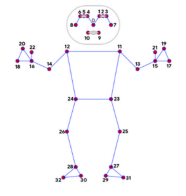
\includegraphics[width=\linewidth]{blazepose.png}
      \caption[BlazePose keypoints]{\label{fig:blazepose}BlazePose keypoints \autocite{RoggioEtAl2024}}
  \end{minipage}
  \hfill % Voegt wat ruimte toe tussen de afbeeldingen
  \begin{minipage}{0.45\textwidth}
      \centering
      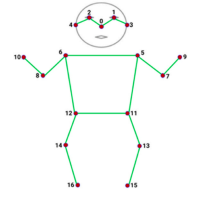
\includegraphics[width=\linewidth]{movenet.png}
      \caption[MoveNet keypoints]{\label{fig:movenet}MoveNet keypoints \autocite{RoggioEtAl2024}}
  \end{minipage}
\end{figure}  

\subsection{Conclusie}
MoveNet Lightning komt als beste keuze naar voren vanwege zijn uitzonderlijke snelheid (>50 FPS) en zijn optimale balans tussen prestaties en nauwkeurigheid. 
Zeker op mobiele apparaten, waar verwerkingscapaciteit en energieverbruik beperkt zijn, maakt deze efficiëntie een belangrijk verschil. 
Vergeleken met MoveNet Thunder, dat iets nauwkeuriger is, maar aanzienlijk trager, blijkt Lightning geschikter voor een realtime analyse-applicatie die feedback moet geven tijdens of vlak na de oefening.

\medskip

Deze configuratie maakt het mogelijk om technische fouten in krachttrainingsoefeningen objectief en onmiddellijk te detecteren, waardoor gebruikers hun uitvoering kunnen verbeteren en blessurerisico’s verlagen.
\chapter{Dataverzameling}
\label{ch:dataverzameling}

Voor deze studie werden meerdere videofragmenten verzameld van drie fundamentele krachtoefeningen: de \textbf{Bench Press}, \textbf{Deadlift} en \textbf{Squat}. 
Elk videofragment werd opgenomen van de \textbf{rechterzijde} van het lichaam van de sporter, zodat de volledige beweging van de rechterkant zichtbaar is tijdens de uitvoering. 
De opnames zijn gemaakt onder gecontroleerde omstandigheden en met een constante camerahoek om uniforme gegevens te waarborgen.

Voor elke oefencategorie zijn zowel correcte als foutieve uitvoeringen geregistreerd. 
De foutieve uitvoeringen werden systematisch gecategoriseerd op basis van biomechanische afwijkingen die visueel detecteerbaar zijn. 
Hieronder worden per oefening de verschillende types afwijkingen beschreven, inclusief de relevante hoeken tussen deze keypoints.

\section{Bench Press}

\subsection*{Correcte Uitvoeringen}
Meerdere correcte uitvoeringen zijn opgenomen waarbij de barbell gecontroleerd naar de borst wordt gebracht en teruggeduwd met een neutrale polspositie, stabiele schouderpositie en volledige \textit{range of motion} (ROM).

\begin{figure}[h]
    \centering
    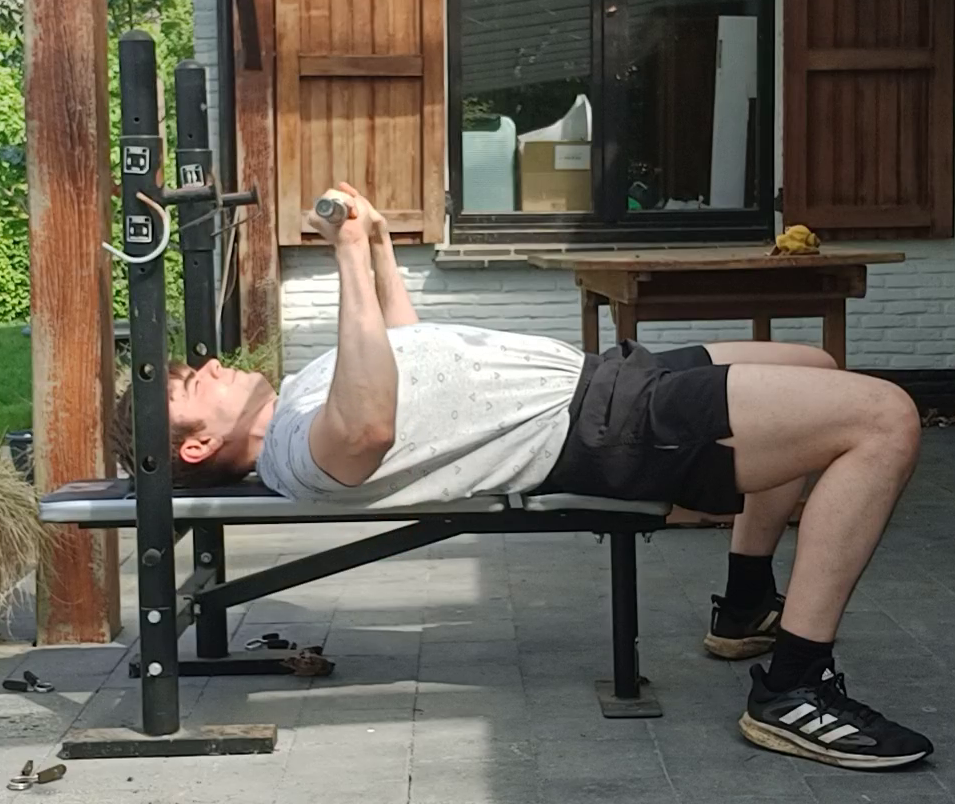
\includegraphics[width=0.5\textwidth]{bench_press_correct.png}
    \caption{Correcte uitvoering van Bench Press (zijaanzicht)}
    \label{fig:bench_correct}
\end{figure}

\subsection{Foutieve Uitvoeringen}
\begin{itemize}
    \item \textbf{Ellebogen te hoog:} Hoek tussen \textit{elleboog–schouder–pols} benadert 180°, wat wijst op een overdreven horizontale armpositie.
    
    \begin{figure}[h]
        \centering
        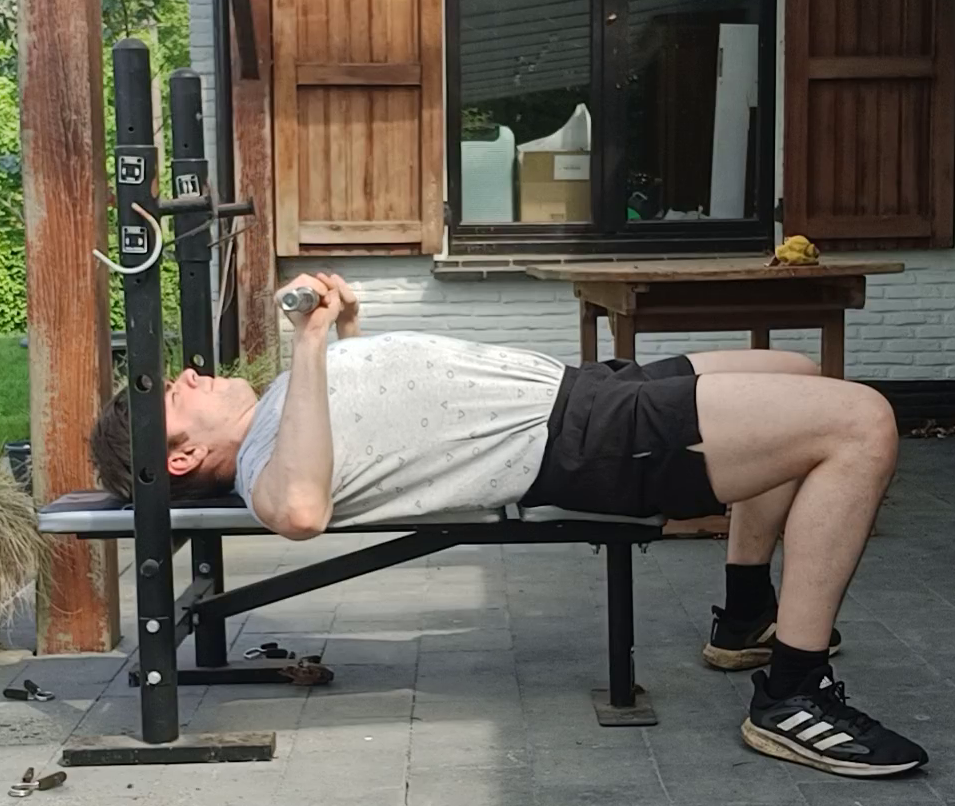
\includegraphics[width=0.5\textwidth]{bench_elbows_high.png}
        \caption{Bench Press met te hoge ellebogen}
        \label{fig:bench_elbows_high}
    \end{figure}
    
    \item \textbf{Te smalle handgreep:} Hoek tussen \textit{ellebogen t.o.v. schouderlijn} is kleiner dan 90°.
    
    \begin{figure}[h]
        \centering
        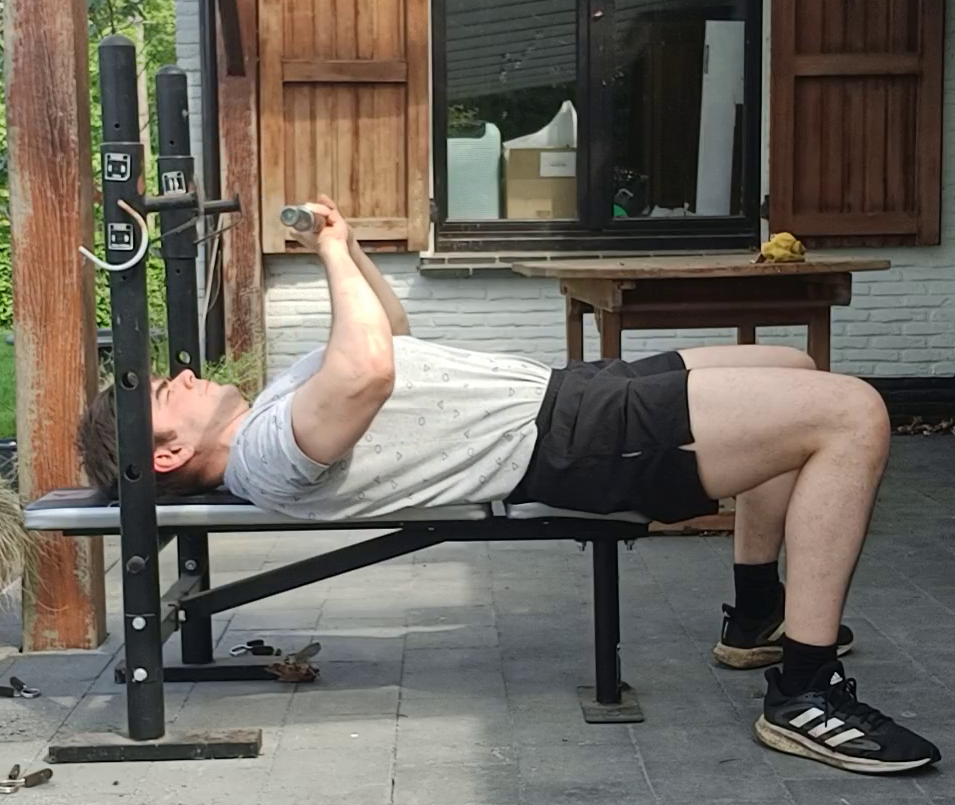
\includegraphics[width=0.5\textwidth]{bench_narrow_grip.png}
        \caption{Bench Press met te smalle handgreep}
        \label{fig:bench_narrow_grip}
    \end{figure}
    
    \item \textbf{Onvolledige herhaling:} Barbell raakt de borst niet; hoek tussen \textit{elleboog–schouder–heup} blijft groter dan 90°.
    
    \item \textbf{Gestrekte knieën:} Hoek tussen \textit{heup–knie–enkel} benadert 180°.
    
    \item \textbf{Pelvis niet op bank:} Afstand tussen heup en bank toont loskomen; hoek \textit{heup–schouder–knie} > 150°.
\end{itemize}

\section{Deadlift}

\subsection{Correcte Uitvoeringen}
De correcte uitvoeringen tonen een rechte rug, neutrale hoofdpositie, stabiele heup-knie-analyse en een verticale barbellbeweging.

\begin{figure}[h]
    \centering
    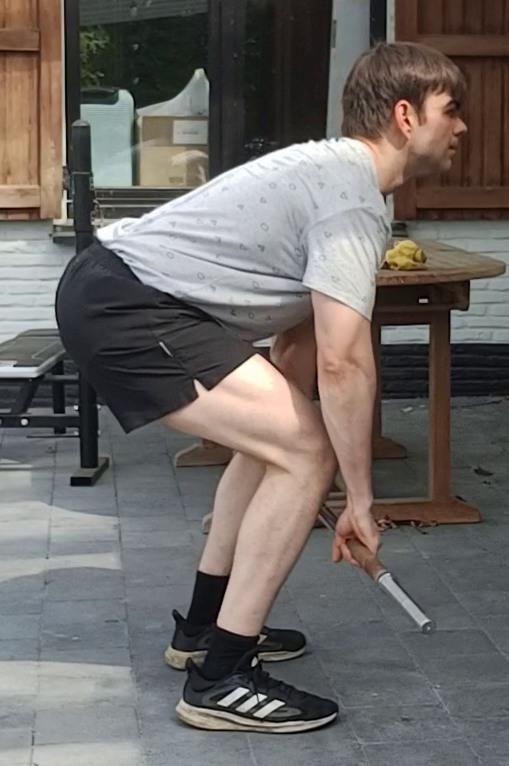
\includegraphics[width=0.5\textwidth]{deadlift_correct.png}
    \caption{Correcte uitvoering van Deadlift}
    \label{fig:deadlift_correct}
\end{figure}

\subsection{Foutieve Uitvoeringen}
\begin{itemize}
    \item \textbf{Kromme rug:} Hoek \textit{schouder–heup–knie} < 160°.
    
    \item \textbf{Te smalle handgreep:} Hoek \textit{elleboog–schouder–elleboog (frontaal)} < 50°.
    
    \item \textbf{Onvolledige herhaling:} Hoek \textit{heup–knie–enkel} blijft > 160°; \textit{schouder–heup–knie} < 180°.
    
    \item \textbf{Te smalle voetstand:} Enkelafstand < heupbreedte; hoek \textit{heup–knie–enkel} vaak < 90°.
    
    \item \textbf{Te brede voetstand:} Enkelafstand > schouderbreedte; resulteert in beperkte ROM.
    
    \item \textbf{Voorover leunen:} Hoek \textit{schouder–heup–enkel} wijkt > 10° af van de verticale as.
\end{itemize}

\begin{figure}[h]
    \centering
    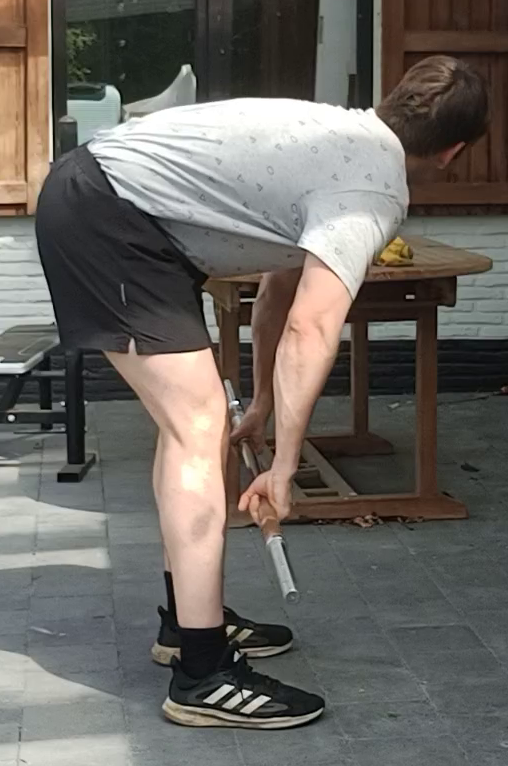
\includegraphics[width=0.5\textwidth]{deadlift_rounded_back.png}
    \caption{Deadlift met kromme rug}
    \label{fig:deadlift_rounded_back}
\end{figure}

\section{Squat}

\subsection{Correcte Uitvoeringen}
De correcte squats tonen diepe bewegingen tot onder parallel, rechte rug en stabiele knie- en enkelpositionering.

\begin{figure}[h]
    \centering
    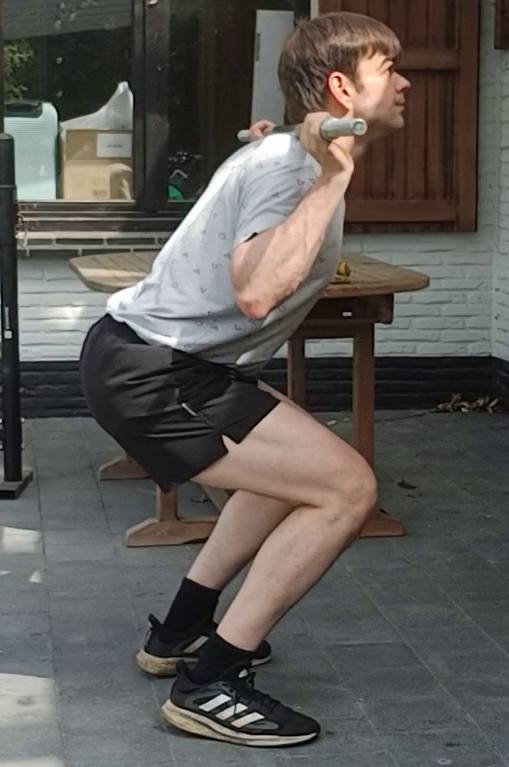
\includegraphics[width=0.5\textwidth]{squat_correct.png}
    \caption{Correcte uitvoering van Squat}
    \label{fig:squat_correct}
\end{figure}

\subsection{Foutieve Uitvoeringen}
\begin{itemize}
    \item \textbf{Kromme rug:} Hoek \textit{schouder–heup–knie} < 160°.
    
    \item \textbf{Onvolledige herhaling:} Hoek \textit{heup–knie–enkel} > 100°, geen diepe squat.
    
    \item \textbf{Te brede voetstand:} Enkelafstand overschrijdt schouderbreedte; hoek \textit{knie–enkel–tenen} > 30°.
\end{itemize}

\begin{figure}[h]
    \centering
    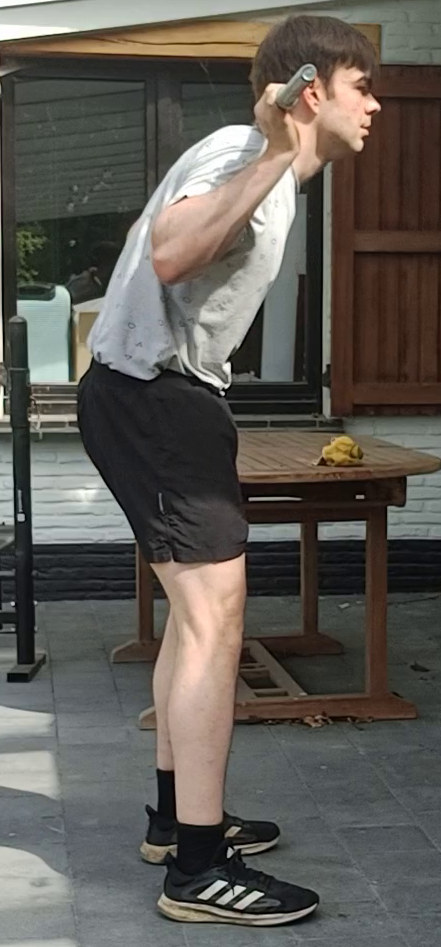
\includegraphics[width=0.5\textwidth]{squat_rounded_back.png}
    \caption{Squat met kromme rug}
    \label{fig:squat_rounded_back}
\end{figure}

\section{Conclusie}
Alle fragmenten zijn zorgvuldig geselecteerd en gecategoriseerd om een evenwichtige dataset te vormen met zowel correcte als incorrecte bewegingspatronen. 

\chapter{Analyse en algoritmische verwerking}
\label{ch:algoritme}

\section{Hoekberekening op basis van keypoints}
Frame per frame worden specifieke hoeken tussen opeenvolgende gewrichten aan de rechterzijde van het lichaam berekend. 
Voor alle drie de geanalyseerde oefeningen — \textit{bench press}, \textit{deadlift} en \textit{squat} —  zijn vier hoeken bijzonder relevant om
 de uitvoering te vergelijken:

\begin{enumerate}
    \item \textbf{Schouder–Elleboog–Pols (SEW)}: \\
    Analyseert de oriëntatie van de onderarm ten opzichte van de bovenarm om bijvoorbeeld een te hoge elleboogpositie of een te smalle grip te detecteren.
    
    \item \textbf{Heup–Knie–Enkel (HKA)}: \\
    Beoordeelt de kniehoek om de diepte van de buiging te meten, belangrijk voor een correcte uitvoering van squat en deadlift.

    \item \textbf{Heup–Schouder–Elleboog (HSE)}: \\
    Meet de hoek bij de oksel om de houding van de bovenarm en romp te evalueren.

    \item \textbf{Schouder–Heup–Knie (SHK)}: \\
    Meet de romphelling en rugintegriteit, cruciaal om een bolle rug te voorkomen bij de deadlift of squat.
\end{enumerate}

Door deze vier hoeken systematisch te berekenen voor elke frame, verkrijgen we een sequentie van hoekwaarden die gebruikt worden voor verdere vergelijkende analyse via \textit{Dynamic Time Warping}.
Bovendien maakt het gebruik van relatieve hoeken een globale normalisatie of het croppen van de poses overbodig. 
Dit betekent dat de hoeken onafhankelijk zijn van de absolute positie of schaal van het skelet in het beeld. 
Hierdoor kunnen verschillende personen en opnames met verschillende camerahoeken of afstanden toch goed met elkaar vergeleken worden.

\section{Dynamic Time Warping}
Een belangrijk probleem bij de vergelijking van twee video’s van dezelfde oefening is het feit dat uitvoeringen kunnen variëren in tempo en startpunt. 
Een sporter kan bijvoorbeeld langzamer of sneller bewegen dan de referentiepersoon, of de beweging kan iets eerder of later starten. 
Hierdoor ontstaat een misalignment in tijd, waardoor een directe frame-per-frame vergelijking onnauwkeurig of misleidend is.
Om dit probleem op te vangen, wordt gebruik gemaakt van het Dynamic Time Warping (DTW) algoritme. 
Dit algoritme zorgt ervoor dat twee reeksen — in dit geval sequenties van lichaamshoeken — optimaal op elkaar worden uitgelijnd, zelfs als de tijdsverdeling ervan ongelijk is. 
DTW berekent het optimale pad tussen deze twee reeksen door een afstandsmatrix op te stellen waarbij elke cel de afstand tussen twee punten in de sequenties representeert. 
Vervolgens zoekt het algoritme naar het pad dat de som van de lokale afstanden minimaliseert, rekening houdend met de mogelijkheid om punten in de sequenties te ‘rekken’ of ‘samentrekken’. 
Zo ontstaat een optimale alignatie van het bewegingsverloop, onafhankelijk van uitvoeringssnelheid of startpunt.

In ons geval gebruikt het Dynamic Time Warping-algoritme de eerder berekende hoekvectoren als invoer. Voor elke cel in de afstandsmatrix wordt de afstand tussen twee frames berekend op basis van de Euclidische afstand tussen de vierdimensionale hoekvectoren:

\[
d(\mathbf{h}_i^A, \mathbf{h}_j^B) = \sqrt{\sum_{k=1}^{4} (\theta_k^i - \theta_k^j)^2}
\]

waarbij $\theta_k^i$ de $k$-de hoekwaarde is in frame $i$ van de referentievideo.

De output is een lijst met frameparen die de uitlijning bepalen:

\[
\text{AlignmentPath} = \left[ (i_1, j_1), (i_2, j_2), \dots, (i_K, j_K) \right]
\]

\section{Vergelijking op basis van hoekverschillen}
Na de temporele uitlijning via DTW worden de hoeken per frame vergeleken. Per framepaar wordt voor elke hoek het verschil berekend:

\[
\text{verschil} = \left| \theta_k^i - \theta_k^j \right|
\]

Dit verschil kan optioneel genormaliseerd worden door deling door 180 graden om een schaal tussen 0 en 1 te verkrijgen, maar kan ook in graden worden behouden. 
Hierbij wordt gebruikgemaakt van de functie \texttt{angleDifferencePerAngle}. Frames waarin bepaalde keypoints ontbreken (en dus alle hoeken nul zijn) worden daarbij uitgesloten.


\section{Conclusie}
Door per frame de relevante hoeken te berekenen, deze te aligneren via \textit{Dynamic Time Warping}, en vervolgens de verschillen te analyseren, ontstaat een robuuste methode om oefeningsuitvoeringen automatisch te vergelijken. 
De focus op hoekvectoren maakt het algoritme ongevoeling voor verschillen in afstand tot de camera, alsook voor verschillen in lichaamsgrootte of -vorm.
Deze aanpak biedt een solide basis voor de verdere ontwikkeling van de proof of concept applicatie, waarin gebruikers hun eigen videofragmenten kunnen vergelijken met referentievideo's om zo hun techniek te verbeteren.



% Voeg hier je eigen hoofdstukken toe die de ``corpus'' van je bachelorproef
% vormen. De structuur en titels hangen af van je eigen onderzoek. Je kan bv.
% elke fase in je onderzoek in een apart hoofdstuk bespreken.

%\input{...}
%\input{...}
%...

%%=============================================================================
%% Conclusie
%%=============================================================================

\chapter{Conclusie}%
\label{ch:conclusie}

% TODO: Trek een duidelijke conclusie, in de vorm van een antwoord op de
% onderzoeksvra(a)g(en). Wat was jouw bijdrage aan het onderzoeksdomein en
% hoe biedt dit meerwaarde aan het vakgebied/doelgroep? 
% Reflecteer kritisch over het resultaat. In Engelse teksten wordt deze sectie
% ``Discussion'' genoemd. Had je deze uitkomst verwacht? Zijn er zaken die nog
% niet duidelijk zijn?
% Heeft het onderzoek geleid tot nieuwe vragen die uitnodigen tot verder 
%onderzoek?

Het doel van dit onderzoek was het ontwikkelen van een mobiele applicatie die krachttrainingsoefeningen automatisch analyseert en objectieve feedback geeft aan de hand van biomechanische parameters. 
Centraal stond de onderzoeksvraag:

\begin{quote}
\textit{Hoe kan een applicatie worden ontwikkeld die bewegingspatronen van cliënten effectief analyseert en vergelijkt met referentievideo’s om nauwkeurige feedback te geven op de uitvoering van krachtoefeningen?}
\end{quote}

Om deze vraag te beantwoorden, werden vier deelvragen geformuleerd. We reflecteren hier op de antwoorden aan de hand van de behaalde resultaten:

\paragraph{1. Welke bestaande technologieën zijn het meest geschikt voor het herkennen en analyseren van menselijke bewegingspatronen in een mobiele applicatie?}
Uit de literatuurstudie en experimentele evaluatie kwam \textbf{MoveNet Lightning} als meest geschikte technologie naar voren. Het model biedt realtime prestaties (>50 FPS) met voldoende nauwkeurigheid (17 keypoints) en kan draaien in de browser via \textbf{TensorFlow.js}, wat compatibel is met een Progressive Web App (PWA). Deze combinatie maakt het mogelijk om zonder installatie of cloudverwerking bewegingsdata te analyseren op mobiele toestellen.

\paragraph{2. Welke parameters zijn het meest relevant voor het nauwkeurig vergelijken van bewegingen tussen de referentievideo en de video van de cliënt?}
Op basis van biomechanische literatuur werden vier kernhoeken gedefinieerd: schouder--elleboog--pols (SEW), heup--knie--enkel (HKA), heup--schouder--elleboog (HSE) en schouder--heup--knie (SHK). Deze hoeken zijn direct gerelateerd aan foutindicatoren zoals bolle rug, onvolledige diepte en slechte elleboogpositie. Het gebruik van deze hoeken maakt het mogelijk om risicovolle afwijkingen automatisch te detecteren, waardoor de app concreet bijdraagt aan blessurepreventie.

\paragraph{3. Hoe kan een algoritme worden ontwikkeld dat verschillen in uitvoering detecteert en bruikbare feedback genereert?}
Het ontwikkelde algoritme combineert \textbf{frame-per-frame hoekberekening} met \textbf{Dynamic Time Warping} (DTW) om temporele verschillen uit te lijnen. Daarna worden de hoeken tussen de referentie- en gebruikersvideo per frame vergeleken, met kleurgecodeerde visuele feedback (groen = correct, rood = afwijking). Deze aanpak bleek effectief bij het identificeren van foutieve houdingen in de bench press, squat en deadlift, zoals geverifieerd in hoofdstuk 8.

\paragraph{4. Hoe kan de nauwkeurigheid van de videovergelijkingen worden getest en gevalideerd?}
De nauwkeurigheid werd geëvalueerd door (1) correcte en incorrecte uitvoeringen met elkaar te vergelijken, (2) identieke video's onderling te vergelijken, en (3) video’s van verschillende lichaamstypes met elkaar te vergelijken. De foutdetectie bleef stabiel met afwijkingen onder 10 graden bij gelijke uitvoeringen en toonde robuuste herkenning van foutpatronen. Hiermee werd de betrouwbaarheid van het algoritme onder reële omstandigheden bevestigd.

\section{Kritische reflectie en beperkingen}

Hoewel de doelen grotendeels zijn bereikt, zijn er enkele belangrijke beperkingen:

\begin{itemize}
    \item De analyse is gebaseerd op video’s vanuit één camerahoek, namelijk de \textbf{rechterzijde}, loodrecht op de sporter. Hierdoor kunnen fouten in het frontale of transversale vlak (zoals rotatie of asymmetrie) niet worden gedetecteerd.
    \item De keypointdetectie is niet-deterministisch; kleine beeldvariaties kunnen leiden tot schommelingen in hoekberekeningen.
    \item Er is nog geen automatische classificatie of concrete coachingfeedback. De gebruiker ziet \textit{waar} afwijkingen optreden, maar niet \textit{hoe} deze te corrigeren zijn.
\end{itemize}

\section{Meerwaarde en bijdrage}

De voorgestelde oplossing draagt concreet bij aan het vakgebied van \textbf{digitale bewegingsanalyse in sport} door:
\begin{itemize}
    \item Een lichtgewicht, toegankelijke oplossing te bieden voor bewegingsfeedback zonder dure apparatuur;
    \item Relevante biomechanische fouten automatisch te detecteren en visueel weer te geven;
    \item Gebaseerd te zijn op robuuste literatuur over blessurepreventie en trainingsoptimalisatie.
\end{itemize}

\section{Aanbevelingen voor toekomstig onderzoek}

Toekomstig onderzoek kan zich richten op:
\begin{enumerate}
    \item \textbf{Multi-view of 3D-analyse} om rotatie en asymmetrieën te detecteren.
    \item \textbf{Automatische foutclassificatie} met tekstuele feedback voor eindgebruikers.
    \item \textbf{Uitgebreid gebruikersonderzoek} met trainers en sporters om de bruikbaarheid en begrijpelijkheid van de feedback te optimaliseren.
    \item \textbf{Testen in realistische omgevingen} met variërende belichting, kleding en camera-afstanden.
\end{enumerate}

\noindent
\textbf{Conclusie:} De combinatie van literatuurgedreven parameters, real-time pose detection en een visueel feedbacksysteem resulteerde in een werkende proof of concept die nauwkeurige, objectieve bewegingsanalyse mogelijk maakt binnen een toegankelijke mobiele applicatie. 
Dit legt een solide basis voor verdere ontwikkeling richting praktische inzetbaarheid in de sport- en revalidatiecontext.




%---------- Bijlagen -----------------------------------------------------------

\appendix

\chapter{Onderzoeksvoorstel}

Het onderwerp van deze bachelorproef is gebaseerd op een onderzoeksvoorstel dat vooraf werd beoordeeld door de promotor. Dat voorstel is opgenomen in deze bijlage.

%% TODO: 
%\section*{Samenvatting}

% Kopieer en plak hier de samenvatting (abstract) van je onderzoeksvoorstel.

% Verwijzing naar het bestand met de inhoud van het onderzoeksvoorstel
%---------- Inleiding ---------------------------------------------------------

% TODO: Is dit voorstel gebaseerd op een paper van Research Methods die je
% vorig jaar hebt ingediend? Heb je daarbij eventueel samengewerkt met een
% andere student?
% Zo ja, haal dan de tekst hieronder uit commentaar en pas aan.

%\paragraph{Opmerking}

% Dit voorstel is gebaseerd op het onderzoeksvoorstel dat werd geschreven in het
% kader van het vak Research Methods dat ik (vorig/dit) academiejaar heb
% uitgewerkt (met medesturent VOORNAAM NAAM als mede-auteur).
% 

\section{Inleiding}%
\label{sec:inleiding}

Met de toenemende aandacht voor fitness en krachttraining is er groeiende vraag naar effectieve, flexibele begeleiding op afstand. Personal trainers en fitnesscoaches zoeken naar manieren om hun cliënten te ondersteunen zonder dat fysieke aanwezigheid vereist is. Videobeelden vormen een unieke kans om de uitvoering van oefeningen nauwkeurig te vergelijken met referentiemateriaal, wat waardevolle feedback inzake de correcte technische uitvoering van deze oefeningen met zich mee brengt.

Traditionele begeleiding beperkt zich vaak tot geschreven instructies of statische afbeeldingen, waardoor nauwkeurigheid in uitvoering ontbreekt en een directe feedbackloop ontbreekt. Dit kan leiden tot onnauwkeurige bewegingen en minder optimale resultaten. Een mobiele applicatie die bewegingspatronen kan analyseren en vergelijken met een referentievideo, zou een doorbraak kunnen betekenen voor zowel zelfstandige personal trainers, alsook fitnesscentra. Het doel van dit onderzoek is dan ook om een gebruiksvriendelijke, technisch haalbare applicatie te ontwikkelen die professionals en cliënten in staat stelt om nauwkeurig bewegingsfeedback te delen. Trainers kunnen een referentievideo van een oefening opnemen en versturen, waarna de cliënt zijn eigen uitvoering filmt. De applicatie vergelijkt de beelden op basis van belangrijke parameters, zoals gewrichtshoeken en bewegingssnelheid, en geeft feedback over de nauwkeurigheid van de uitvoering.

De centrale onderzoeksvraag luidt als volgt:

\begin{itemize}
  \item Hoe kan een applicatie worden ontwikkeld die bewegingspatronen van cliënten effectief analyseert en vergelijkt met referentievideo’s om nauwkeurige feedback te geven op de uitvoering van krachtoefeningen?
\end{itemize}

Om deze hoofdvraag te kunnen beantwoorden dien de volgende deelvragen eerst aangepakt te worden:

\begin{itemize}
  \item Welke bestaande technologieën zijn het meest geschikt voor het herkennen en analyseren van menselijke bewegingspatronen in een mobiele applicatie?
  \item Welke parameters zijn het meest relevant voor het nauwkeurig vergelijken van bewegingen tussen de referentievideo en de video van de cliënt?
  \item Hoe kan een algoritme worden ontwikkeld dat verschillen in uitvoering detecteert en bruikbare feedback genereert?
  \item Hoe kan de nauwkeurigheid van de deze videovergelijkingen worden getest en gevalideerd?
\end{itemize}

%---------- Stand van zaken ---------------------------------------------------

\section{Literatuurstudie}%
\label{sec:literatuurstudie}


Een goede techniek bij het uitvoeren van kracht- en revalidatieoefeningen zorgt er niet alleen voor dat de juiste spieren en gewrichten worden geactiveerd. Het leidt tevens tot een verminderd risico op acute blessures, zoals verrekkingen of spierscheuren. Het is dus noodzakelijk dat men een goede techniek wordt aangeleerd aan de hand van voortdurende en directe feedback. Voor deze feedback kan er met beeldmateriaal gewerkt worden, wat dan weer de deur opent tot ondersteuning vanop afstand\autocite{MyerEtAl2009}.

\emph{Human Pose Estimation} is een technologie die de positie en oriëntatie van een menselijk lichaam in een afbeelding of video analyseert en weergeeft. Het doel van \emph{human pose estimation} is om belangrijke punten van het lichaam, zoals de ogen, neus, schouders, ellebogen, polsen, heupen, knieën en enkel, te identificeren en in kaart te brengen, waardoor een digitaal skelet ontstaat dat de houding of beweging van de persoon in real-time kan volgen. Achterliggend maakt deze technologie gebruik van \emph{Deep Learning}, een onderdeel van \emph{machine learning} dat gebruikt maakt van kunstmatige neurale netwerken om complexe data te verwerken\autocite{JosyulaEtAl2021}.

Tegenwoordig worden er al vaak Pose Estimation frameworks succesvol gebruikt voor de analyse van een menselijke houding. Zo haalde het gebruikte model van \textcite{ParasharEtAl2023} een accuraatheid van 99.50\% bij de herkenning van 5 verschillende yoga posities.


% Voor literatuurverwijzingen zijn er twee belangrijke commando's:
% \autocite{KEY} => (Auteur, jaartal) Gebruik dit als de naam van de auteur
%   geen onderdeel is van de zin.
% \textcite{KEY} => Auteur (jaartal)  Gebruik dit als de auteursnaam wel een
%   functie heeft in de zin (bv. ``Uit onderzoek door Doll & Hill (1954) bleek
%   ...'')


%---------- Methodologie ------------------------------------------------------
\section{Methodologie}%
\label{sec:methodologie}
\subsection{Vergelijkend onderzoek}
\label{sec:vergelijkend onderzoek}

Vooreerst zal een een literatuurstudie worden uitgevoerd om de verschillende, meest gebruikte, Pose Estimation frameworks in kaart te brengen. Deze worden vervolgens tegenover elkaar afgewogen op basis van gebruiksvriendelijkheid, precisie en snelheid. Mogelijks komen er uit de literatuurstudie nog parameters naar boven die ook in deze afweging kunnen opgenomen worden. Naast een uiteenzetting van de verschillende Pose Estimation frameworks, zal er ook onderzocht worden welke krachttrainingsoefeningen het meest prevalent zijn. Op basis hiervan wordt de data in de volgende fase gekozen. Deze fase zal een tweetal weken in beslag nemen.

\subsection{Dataverzameling}
\label{sec:dataverzameling}

In de tweede fase wordt er beeldmateriaal van de geselecteerde oefeningen verzameld en gelabeld. Hiervoor zal voornamelijk gebruik gemaakt worden van online beschikbaar beeldmateriaal. Deze fase zal ongeveer vier weken in beslag nemen.

\subsection{Ontwikkeling van het model}
\label{sec:ontwikkeling van het model}

Hierin wordt een \emph{Deep Learning} model ontwikkeld en getraind op basis van de aangelegde dataset. Bij afloop van deze fase beschikken we bijgevolg over een model dat in staat is de geselecteerde krachtoefeningen te herkennen. Deze fase zal ongeveer drie weken duren.

\subsection{Testen van het model}
\label{sec:testen van het model}
Het model wordt getest met een deel van de eerder verzamelde data, die niet gebruikt werd tijdens het trainen van het model. Deze fase zal ongeveer een week duren.

\subsection{Ontwikkeling van de mobiele applicatie}
\label{sec:ontwikkeling van de mobiele applicatie}
Er wordt een mobiele applicatie ontwikkeld waarbij de client persoonlijk videomateriaal kan toetsen aan het getraind model en zodoende feedback verkrijgt over de houding tijdens de uitvoering van de krachtrainingsoefening. Dit zal een drietal weken in beslag nemen.

%---------- Verwachte resultaten ----------------------------------------------
\section{Verwacht resultaat, conclusie}%
\label{sec:verwachte_resultaten}

De ontwikkelde applicatie zal gebruikers in staat stellen om videobeelden van krachtoefeningen eenvoudig en effectief te vergelijken met referentiemateriaal. Door gebruik te maken van geavanceerde pose estimation en een specifiek ontwikkeld algoritme voor bewegingsanalyse, biedt de applicatie gedetailleerde en nauwkeurige feedback over de technische uitvoering van oefeningen. Deze feedback is gericht op het verbeteren van bewegingspatronen, het minimaliseren van blessures en het optimaliseren van trainingsresultaten.

Het onderzoek zal naar verwachting aantonen welke pose estimation framework het meest geschikt is voor het ontwikkelen van een toegankelijke en gebruiksvriendelijke mobiele applicatie. Bovendien zullen de bevindingen inzicht geven in de relevante parameters voor bewegingsvergelijking en hoe deze effectief kunnen worden toegepast om real-time feedback te genereren. De resultaten dragen niet alleen bij aan de fitness- en trainingssector, maar bieden ook een solide basis voor bredere toepassingen, zoals revalidatie en preventieve zorg, waarin bewegingsanalyse een cruciale rol speelt.



%%---------- Andere bijlagen --------------------------------------------------
% TODO: Voeg hier eventuele andere bijlagen toe. Bv. als je deze BP voor de
% tweede keer indient, een overzicht van de verbeteringen t.o.v. het origineel.
%\input{...}

%%---------- Backmatter, referentielijst ---------------------------------------

\backmatter{}

\setlength\bibitemsep{2pt} %% Add Some space between the bibliograpy entries
\printbibliography[heading=bibintoc]

\end{document}
